%%%%%%%%%%%%%%%%%%%%%%%%%%%%%%%%%%%%%%%%%
% Beamer Presentation
% LaTeX Template
% Version 1.0 (10/11/12)
%
% This template has been downloaded from:
% http://www.LaTeXTemplates.com
%
% License:
% CC BY-NC-SA 3.0 (http://creativecommons.org/licenses/by-nc-sa/3.0/)
%
%%%%%%%%%%%%%%%%%%%%%%%%%%%%%%%%%%%%%%%%%

%----------------------------------------------------------------------------------------
%	PACKAGES AND THEMES
%----------------------------------------------------------------------------------------
\PassOptionsToPackage{subsection=false}{beamerouterthememiniframes}
\documentclass{beamer}
\usepackage{listings}
\usepackage{mdframed}

\renewcommand{\figurename}{Figure}
\renewcommand{\tablename}{Table}
\renewcommand{\lstlistingname}{Code Snippet} 

\def\titulo{{Securing openHAB Smart Home through User Authentication and Authorization}}
\def\autor{Jes\'{u}s Antonio Soto Vel\'{a}zquez}
\def\grado{Master of Science in Engineering (Computer Science)}
\def\matricula{B70630}
\def\fecha{June 2018}
\usepackage[numbers,sort]{natbib}
%\bibliographystyle{../estiloDeBibliografia}

\setbeamertemplate{caption}[numbered]


\definecolor{carolinablue}{rgb}{0.6, 0.73, 0.89}
\definecolor{lbcolor}{rgb}{0.9,0.9,0.9}
\lstset{
    tabsize=4,    
    language=Java,
    basicstyle=\scriptsize,
    upquote=true,
    %        aboveskip={1.5\baselineskip},
    columns=fixed,
    showstringspaces=false,
    extendedchars=false,
    breaklines=true,
    prebreak = \raisebox{0ex}[0ex][0ex]{\ensuremath{\hookleftarrow}},
    frame=single,
    numbers=left,
    numberstyle=\tiny,
    numbersep=5pt,
    showtabs=false,
    showspaces=false,
    showstringspaces=false,
    identifierstyle=\ttfamily,
    keywordstyle=\color[rgb]{0.0, 0.45, 0.73},
    commentstyle=\color[rgb]{0.09, 0.45, 0.27},
    stringstyle=\color[rgb]{0.627,0.126,0.941},
%    numberstyle=\color[rgb]{0.205, 0.142, 0.73},
    %        \lstdefinestyle{C++}{language=C++,style=numbers}’.
}


\mode<presentation> {
  \usetheme{Berlin}
  \usecolortheme{spruce}
%\useoutertheme[subsection=false]{miniframes}

%\setbeamertemplate{footline} % To remove the footer line in all slides uncomment this line
\setbeamertemplate{footline}[page number] % To replace the footer line in all slides with a simple slide count uncomment this line

%\setbeamertemplate{navigation symbols}{} % To remove the navigation symbols from the bottom of all slides uncomment this line
}

\usepackage{graphicx} % Allows including images
\graphicspath{{../fig/}}
\usepackage{booktabs} % Allows the use of \toprule, \midrule and \bottomrule in tables



%----------------------------------------------------------------------------------------
%	TITLE PAGE
%----------------------------------------------------------------------------------------

\title[]{\titulo} % The short title appears at the bottom of every slide, the full title is only on the title page

\author{\autor} % Your name
\institute[UT]{
  UNIVERSITY OF TARTU\\[3mm]
  Institute of Computer Science\\
  Computer Science Curriculum\\[3mm]  
  
\includegraphics[height=3cm]{UT_logo}
}

\date{\fecha} % Date, can be changed to a custom date

\begin{document}

\begin{frame}
\titlepage % Print the title page as the first slide
\end{frame}

\begin{frame}
\frametitle{Overview} % Table of contents slide, comment this block out to remove it
\tableofcontents % Throughout your presentation, if you choose to use \section{} and \subsection{} commands, these will automatically be printed on this slide as an overview of your presentation
\end{frame}

%----------------------------------------------------------------------------------------
%	PRESENTATION SLIDES
%----------------------------------------------------------------------------------------

%------------------------------------------------
\section{Introduction} % Sections can be created in order to organize your presentation into discrete blocks, all sections and subsections are automatically printed in the table of contents as an overview of the talk
%------------------------------------------------
\begin{frame}
\frametitle{Introduction: Internet of Things}
\textbf{Internet of Things.} Dynamic and heterogenous environment where \emph{sensing} devices interact with each other. 
\begin{itemize}
\setlength\itemsep{1.5em}
\item Devices: smartphones, smart watches, smoke alarm, security camera, heartbeat and temperature monitor, etc.
\item Applications: Smart home, smart city, smart healthcare, intelligent transportation, etc.
\item Challenges: interoperability, architecture, device naming, usability, security and privacy.  
\end{itemize}
\end{frame}
%------------------------------------------------
\begin{frame}
\frametitle{A Smart Home Application: OpenHAB}
\textbf{``a vendor and technology agnostic open source automation software for your home''} (openHAB Community, 2010)
\begin{itemize}
  \setlength\itemsep{1.5em}
\item May be deployed on very modest devices (e.g., Raspberry Pi)
\item Mostly works without an Internet connection.
\item Uses thing-specific \emph{bindings} to connect to devices.
\item Made up of individual projects, e.g.\ Eclipse SmartHome.
\item Written in Java under the OSGi architecture. 
\end{itemize}
\end{frame}
%------------------------------------------------
\begin{frame}
\frametitle{Objectives} % objectives?
\begin{enumerate}
  \setlength\itemsep{1.5em}
\item To analyze the security mechanisms in use for the openHAB automation software.
\item To implement an authenticator based on the JSON Web Token for Eclipse Smarthome.
\item To propose a fine-grained, yet usable authorization model for openHAB to manage usage permissions.
\end{enumerate}
\end{frame}
%------------------------------------------------
\begin{frame}
\frametitle{Motivation}
\begin{itemize}
  \setlength\itemsep{1.5em}
\item Developments of IoT applications focus mostly on functional requirements, leaving usability, performance, security, etc., for later.
\item Consequences in smart home range from mere user discomfort to identity theft, or worse.
\item Lack of security deters adoption of IoT applications, halts progress. 
\end{itemize}
\end{frame}
%------------------------------------------------
\section{Security Challenges in OpenHAB}
\begin{frame}
\frametitle{Security Challenges in OpenHAB}
\begin{itemize}
  \setlength\itemsep{1.5em}
\item Intranet of Things
\item Bindings
\item Access Control
\end{itemize}
\end{frame}
%------------------------------------------------
\begin{frame}
\frametitle{Intranet of Things}
\begin{itemize}
  \setlength\itemsep{1.5em}
\item Aims to contain private data locally.
\item Puts a limitation on use cases.
\item Secure remote access: a challenge.
\item Assumes security of the private network.
\end{itemize}
\end{frame}
%------------------------------------------------
\begin{frame}
\frametitle{Security of Bindings}
\textbf{Binding.} Logical modules to support inter-device interaction inside openHAB.
\begin{itemize}
  \setlength\itemsep{1.5em}
\item Each binding is defined for things that use a certain protocol, e.g.: KNX, Z-Wave, ZigBee, Panasonic TV, etc.
\item Some bindings use an API for remote connection to the vendor.
\item Remote communication may be done under HTTPS if specified by binding.
\end{itemize}
\end{frame}
%------------------------------------------------
\begin{frame}
\frametitle{Access Control}
\begin{itemize}
  \setlength\itemsep{1.5em}
\item Whoever gains access to private network gains access to smart home management.
\item Not trivial: previous attempts have failed.
\item To be implemented inside the core framework: Eclipse SmartHome.
\item Main challenge: single \emph{authentication context} recognizable in all end points (servlets).
\end{itemize}
\end{frame}
%------------------------------------------------
\begin{frame}
\frametitle{Misuse Cases}

\begin{figure} [ht] 
\begin{center}
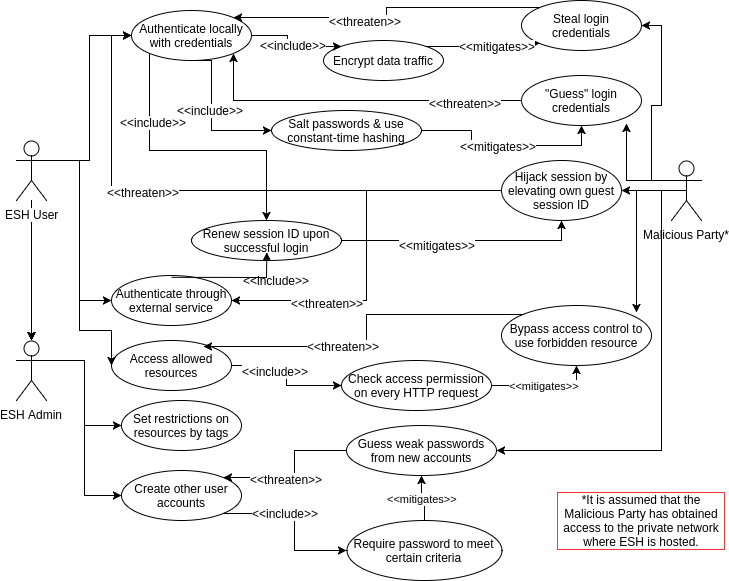
\includegraphics[width=0.75\textwidth]{esh_misuse_cases}
\caption{Misuse Cases for Access Control in ESH.}
\label{fig:misuse_cases}
\end{center}
\end{figure}

\end{frame}
%------------------------------------------------
\section{Proposed Security Mechanisms}
\begin{frame}
\frametitle{Proposed Security Mechanisms}
\begin{itemize}
  \setlength\itemsep{1.5em}
\item JSON Web Token-based Authenticator
\item RBAC-inspired Authorization Model
\end{itemize}
\end{frame}
%------------------------------------------------
\begin{frame}
\frametitle{JSON Web Token Structure}
\begin{enumerate}
  \setlength\itemsep{1.5em}  
\item Header: type of token (JWT), hashing algorithm (e.g., HMAC SHA256, RSA).
\item Payload: claims about the user (e.g., username, roles).
\item Signature: Using a secret key creates a signature of the previous parts.
\end{enumerate}
\end{frame}
%------------------------------------------------
\begin{frame}
\frametitle{Token-based Authentication Procedure}
\begin{figure} [ht] 
\begin{center}
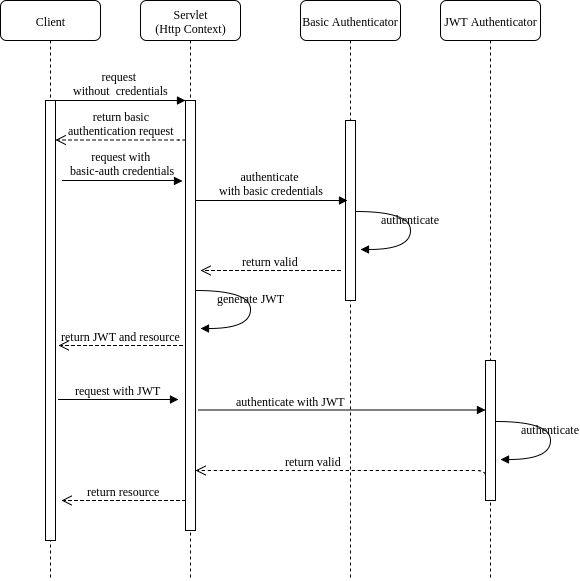
\includegraphics[width=0.6\textwidth]{esh_auth_sequence}
\caption{Addition of authenticators into the architecture.}
\label{fig:esh_arch_authenticator}
\end{center}
\end{figure}
\end{frame}
%------------------------------------------------
\begin{frame}
\frametitle{Architectural Implications}
\begin{figure} [ht] 
\begin{center}
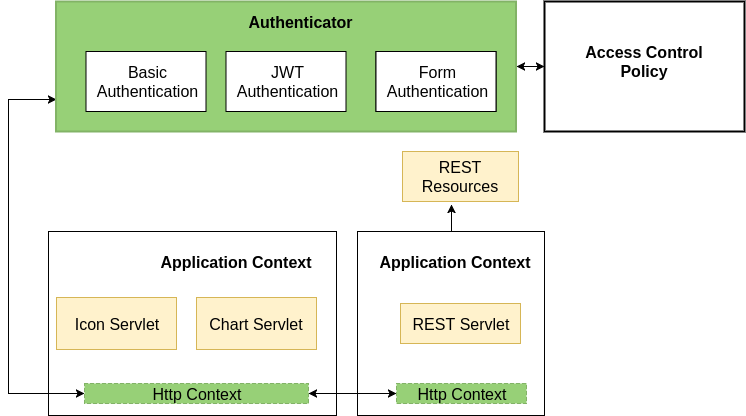
\includegraphics[width=0.8\textwidth]{esh_arch_authenticator}
\caption{Addition of authenticators into the architecture.}
\label{fig:esh_arch_authenticator}
\end{center}
\end{figure}
\end{frame}
%------------------------------------------------
\begin{frame}
\frametitle{Implementation of Authenticators}
Some remarks:
\begin{itemize}
  \setlength\itemsep{1.5em}
\item Prepared to work for a \emph{shared} authentication context.
\item \emph{JWT} authentication when token is provided in request (cookie or HTTP header).
\item Nimbus used as JWT library. 
\item RSA key pair is created during runtime and stored in memory. 
\item \emph{Basic} authentication (username:password) as fallback authentication mechanism.
\item Registration to OSGi 4.2 runtime is done differently than in OSGi 6 runtime. 
\end{itemize}
\end{frame}
%------------------------------------------------
\begin{frame}
\frametitle{Proposed Authorization Model}
\begin{itemize}
  \setlength\itemsep{1.5em}
\item As a smart home application, an authorization model should be fine grained and usable.
\item Tasks that may be done on openHAB are grouped as \emph{capability sets}.
\item Registered users are assigned one or more capability sets to reflect their privilege in the system.
\item Permissions range from: REST endpoints, sitemaps, traditional servlets, automation rules, third-party add-ons, system settings, etc.
\end{itemize}
\end{frame}
%------------------------------------------------
\begin{frame}
\frametitle{User-Assigned Capability Sets}
\begin{table}[h]
  \centering
  \caption{Sample relation of user and capability sets}
  \begin{tabular}{|l|l|}
    \hline
    \multicolumn{1}{|c|}{\textbf{User}} & \multicolumn{1}{c|}{\textbf{Capability Sets}}            \\ \hline
    Marian                              & (speakers-quiet, lights-on, doors-close, sitemaps-paper) \\ \hline
    Erika                               & (speakers-playback, lights-all, doors-all, sitemaps-all) \\ \hline
  \end{tabular}
  \label{tbl:autho_cap}
\end{table}

\begin{table}[h]
  \centering
  \caption{Sample listings of operations involved for each capability set}  
  \begin{tabular}{ll}
    \hline
    \multicolumn{1}{|c|}{\textbf{Capability Set}} & \multicolumn{1}{c|}{\textbf{Involved Operations}}                                                                                                                                                                                      \\ \hline
    \multicolumn{1}{|l|}{speakers-playback}   & \multicolumn{1}{l|}{\begin{tabular}[c]{@{}l@{}}yamahareceiver.internal.state.\\NavigationControlState.getCurrentItemName()\\ ZoneControlState.volume\end{tabular}} \\ \hline
    \multicolumn{1}{|l|}{things-all}          & \multicolumn{1}{l|}{\begin{tabular}[c]{@{}l@{}}rest.core.internal.thing.ThingResource.getAll()\\ rest.core.internal.thing.ThingResource.create()\end{tabular}}                       \\ \hline
    &
  \end{tabular}
  \label{tbl:autho_op}
\end{table}

\end{frame}
%------------------------------------------------
\begin{frame}
\frametitle{Evaluation}
Authenticator was evaluated in two OSGi runtimes: Karaf (Apache Felix), and Eclipse SmartHome (Eclipse Equinox).
\begin{enumerate}
  \setlength\itemsep{1.5em}
\item Karaf deployment supported OSGi R6. \\ Servlet and context registration was made through Whiteboard pattern. 
\item ESH deployment supported up to OSGi R4.2. \\ Servlet and context registration was made through \texttt{Http Service} and \texttt{Http Tracker}. 
\end{enumerate}
\end{frame}
%------------------------------------------------
\section{Conclusion and Future Research Directions}
\begin{frame}
\frametitle{Conclusion}
Contributions:
\begin{itemize}
  \setlength\itemsep{1.5em}
\item Analysis of the security mechanisms in use for the openHAB automation software.
\item Implementation of a client authenticator based on the JSON Web Token for Eclipse Smarthome.
\item Proposal of a fine-grained, yet usable authorization model for openHAB to manage usage permissions.
\end{itemize}
\end{frame}
%------------------------------------------------
\begin{frame}
\frametitle{Future Research Directions}
\begin{itemize}
  \setlength\itemsep{0.9em}
\item Incorporation of form-based authentication in the OSGi architecture.
\item Expiration and renewal of JWT issued by Eclipse SmartHome.
\item Encryption of JWT.
\item Unique generation and storage RSA key pair.
\item Local storage of user credentials (e.g., LDAP).
\item Integration with external authentication providers (e.g., OAuth).
\item Design access for first-time users.
\item Implementation of the proposed authorization model.
\end{itemize}

\end{frame}
%------------------------------------------------
% REFERENCES? no~
\end{document}
